\chapter{CCMail}
\label{cha:ccmail}
In diesem Kapitel wird die existierende Anwendung \emph{CCMail} analysiert und diskutiert. Ziel ist es einen Überblick über diese Anwendung und dessen Aspekte zu liefern sowie diese Aspekte genauer zu betrachten und zu analysieren. Die Ergebnisse dieser Analyse sollen als Grundlage für das neue Konzept dienen, dass auch die Integration in die bestehenden Anwendungen berücksichtigen muss. Diese Integration soll natürlich mit geringstem Aufwand erfolgen können, da hier Probleme bei der Integration negative Auswirkungen auf den produktiven Betrieb haben könnten. 

\section{Systemaufbau}
\label{sec:ccmail-systemaufbau}
Im folgenden wird der Systemaufbau aus der Sicht der Anwendung \emph{CCMail} und dessen Integration in das System diskutiert. 
\begin{figure}[h]
\centering
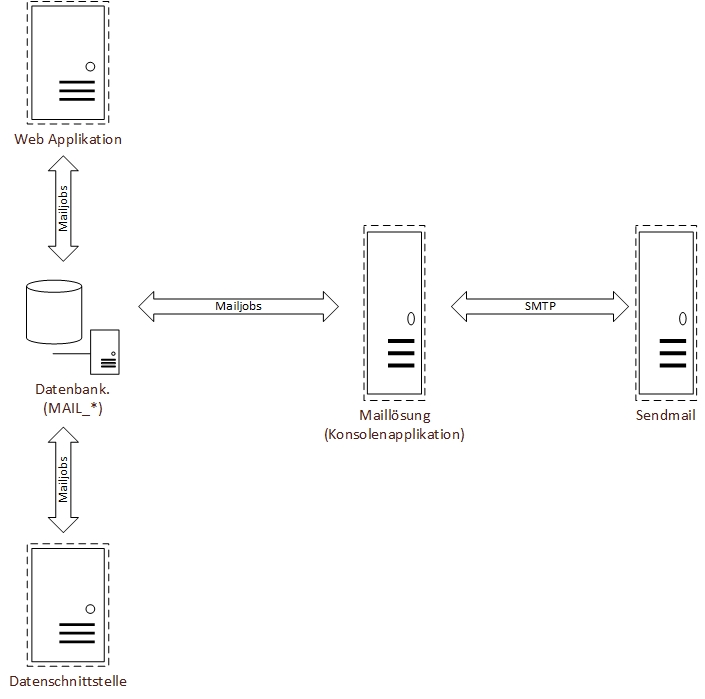
\includegraphics[scale=0.35]{Systemaufbau_alt.jpg} %{CS0031}
\caption{Systemaufbau und Integration von \emph{CCMail}}
\label{fig:ccmail-system-und-integration}
\end{figure}
\ \newpage
\parindent0pt{Dieses} Diagramm zeigt das Gesamtsystem aus der Sicht der Anwendung \emph{CCMail}, wobei anzumerken ist, dass das System bis heute angewachsen ist und nunmehr aus mehreren Anwendungen besteht. Es lässt sich hier ableiten dass das Kernstück des Systems die Datenbank ist. In der Datenbank werden die zu versendenden E-Mail-Nachrichten als sogenannte \emph{MailJobs} verwaltet. Ein \emph{MailJob} ist ein Eintrag in einer Datenbanktabelle namens \emph{MAIL\_JOBS}, die alle Informationen einer E-Mail-Nachricht enthält. Hierbei sind die eigens implementierten Datenbankzugriffsschichten zu kritisieren, die zwar den Datenbankzugriff kapseln, jedoch nur für jede Anwendung an sich und nicht über Anwendungsgrenzen hinweg, was durchaus möglich wäre. Scott W.Ambler und Parmod J.Sadalge beschreiben es in Ihrem Buch \cite[27]{refactoreDatabase} treffend:
\begin{quote}
\emph{The greather the coupeling, the harder is to refactore something. This is true of code refactoring, and it is certainly true of database refactoring}
\end{quote}
Da jede Anwendung ihre eigene Datenzugriffsschicht hält, muss jede Anwendung bei einer Datenbankänderung ihre Datenzugriffsschicht anpassen. Eine zentrale Datenbankzugriffsschicht würde nur eine Änderung an einer Seite erfordern. Also haben wir hier eine Form der starken Koppelung die sich durch die Code-Duplikate ausprägt.
\newline
\newline
Die Anwendungen \emph{CleverWeb} und \emph{CleverInterface} erstellen über ihre eigens implementierte Datenbankzugriffsschicht \emph{MailJob} Entitäten in der Datenbank, welche zeitgesteuert von \emph{CCMail} ausgelesen, verarbeitet und versendet werden. \emph{CCMail} ist als eine Konsolen-Anwendung Implementiert und enthält alle Ressourcen, die es benötigt um die \emph{MailJob} Entitäten zu verarbeiten. Auch hier wirken sich die eigens implementierten Datenbankzugriffsschichten aus, da es hier keine einheitliche Spezifikation für das Erstellen eines \emph{MailJobs} gibt. Validierungen ob ein zu erstellender \emph{MailJob} gültig ist wird hier den einzelnen Anwendungen überlassen und sind nicht an einer zentralen Stelle spezifiziert. Daher muss sich die Implementierungen in \emph{CCMail} darauf verlassen, dass alle Anwendungen die \emph{MailJobs} korrekt anlegen damit diese von \emph{CCMail} korrekt verarbeitet werden können.
\newline
\newline
Als Mail-Server wird \emph{Sendmail} verwendet. Es handelt sich hierbei um eine Anwendung, die für Linux Distributionen frei verfügbar ist. \emph{CCMail} versendet über das SMTP-Protokoll die E-Mail-Nachrichten an die \emph{Sendmail} Instanz, die sie ihrerseits an die EmpfängerInnen versendet.

\newpage
\section{E-Mail-Versand}
\label{sec:ccmail-email-versand}
Der folgend beschriebene Prozess des E-Mail-Versandes soll aufzeigen wie in dem vorherig beschriebenen System \ref{sec:ccmail-systemaufbau} der E-Mail-Versand vom Anlegen eines \emph{MailJob} bis hin zum Versand der eigentlichen E-Mail-Nachricht funktioniert. Als Kernkomponente des Systems wurde die Datenbank identifiziert, die die \emph{MailJob} Entitäten hält, die wiederum von \emph{CCMail} aus der Datenbank ausgelesen und verarbeitet werden. Dieser Ansatz ist an sich nicht als schlecht anzusehen, jedoch verbirgt sich hier eines der Hauptprobleme des E-Mail-Versandes. Nämlich die Inkonsistenz der versendeten E-Mail-Nachrichten, durch die Zeitdifferenz zwischen dem Anlegen eines \emph{MailJob} durch die Anwendungen und dem tatsächlichen Versand der E-Mail-Nachricht durch \emph{CCMail}.
\begin{figure}[h]
\centering
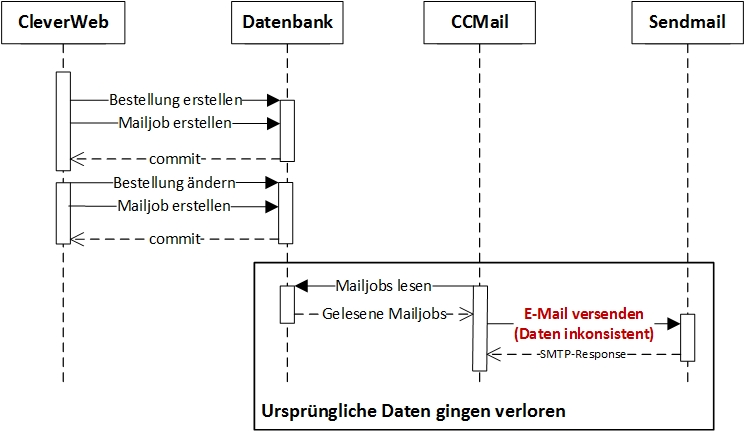
\includegraphics[scale=0.8]{prozess_sequence_emailversand.jpg}
\caption{Gesamtprozess des E-Mail Versandes}
\label{fig:sequence-diagramm-gesamtprozess}
\end{figure}
\ \newline
Wie man aus dem Sequenz Diagramm ableiten kann ist eines der Hauptprobleme am E-Mail-Versand die Inkonsistenz, was in der Art und Weise wie die \emph{MailJob} Entitäten verarbeitet werden begründet ist. Aufgrund der zeitgesteuerten bzw. zeitversetzten Verarbeitung kann es vorkommen dass sich die zugrunde liegenden Daten einer E-Mail-Nachricht ändern bevor diese überhaupt versendet wurde. In diesem Beispiel wird eine Bestellung angelegt und kurz darauf geändert. Dies geschieht bevor die E-Mail-Nachricht über das Anlegen der Bestellung versendet wurde. Es wurde zwar ein neuer \emph{MailJob} angelegt aber beide \emph{MailJob} Einträge verweisen auf dieselbe Bestellung. Dadurch enthalten beide versendeten E-Mail-Nachrichten dieselben Informationen und die Informationen der ursprünglich erstellten Bestellung gingen verloren. 
\newline
\newline
Dies ist begründet in der Art und Weise wie die \emph{MailJob} Einträge aufgebaut sind. Ein \emph{MailJob} hält die Informationen für den Versand einer E-Mail wobei hierbei nicht die gesamte E-Mail-Nachricht oder die verwendeten Daten gespeichert werden, sondern lediglich die Parameter, die in einer SQL-Abfrage benutzt werden, um die Daten für die E-Mail-Nachricht zu erhalten. Sollten sich also die Datenbank Entitäten der involvierten Tabellen ändern so sind die ursprünglichen Daten nicht mehr wiederherstellbar. Dadurch ist auch ein erneuter Versand einer bereits versendeten E-Mail-Nachricht nicht mehr möglich bzw. es kann nicht garantiert werden, dass diese Nachricht dieselben Informationen enthält wie beim ersten Versand.
\newline
\newline
Ein Weiteres Problem liegt in der zeitgesteuerten Verarbeitung der \emph{MailJob} durch \emph{CCMail}. Es wurde lange Zeit nicht geprüft ob bereits ein \emph{CCMail} Prozess gestartet wurde bevor dieser gestartet wird. Dies hat dazu geführt dass es vorkam das mehrere Prozesse gleichzeitig die \emph{MailJob} Entitäten verarbeiten und daher die E-Mail-Nachrichten mehrmals versendet wurden. Dieses Problem ist begründet durch die Tatsache dass in Verarbeitung stehende \emph{MailoJob} Entitäten nicht als \emph{"In Progress"} markiert wurden und von dem parallel laufende Prozess ebenfalls ausgelesen und verarbeitet wurden. Zurzeit wird lediglich geprüft ob bereits ein Prozess gestartet wurde, was es unmöglich macht die Arbeit auf mehrere Prozesse aufzuteilen. Dies hat zur Folge dass der E-Mail-Versand seriell verläuft obwohl angemerkt sei, dass die einzelnen Nachrichten sehr wohl parallel in eigenen Threads verarbeitet und versendet werden. Nicht desto Trotz könnte man hier die Arbeit auf mehrere Prozesse aufteilen und so die Performance verbessern und den Zeitaufwand für den Versand minimieren.

\newpage
\section{Software-Design}
\label{sec:ccmail-software-design}
Nachdem der Systemaufbau diskutiert wurde wird sich nun mit dem Software-Design von \emph{CCMail} befasst. \emph{CCMail} wurde als Konsolen-Anwendung implementiert und hält alle Ressourcen, die zur Verfügung stehen wie:
\begin{enumerate}
	\item E-Mail-Vorlagen
	\item Datenbankabfragen
	\item E-Mail-Typ spezifische Implementierungen
\end{enumerate}
\ \newline
Als Kernpunkt der Anwendung bzw. dessen Implementierungen ist die Klasse \emph{CCBasicEmail} anzusehen, die die gesamte Funktionalität für den Versand einer E-Mail-Nachricht enthält, sowie eine Klasse namens \emph{CCMailingDao} die alle Datenbankabfragen über alle E-Mail-Typen hinweg enthält.
\begin{figure}[h]
\centering
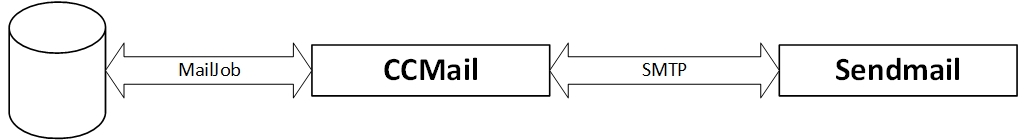
\includegraphics[scale=0.5]{teilsystem_ccmail.jpg} 
\caption{Teilsystem \emph{CCMail}}
\label{fig:ccmail-teilsystem}
\end{figure}
\ \newline
Dieser Teil soll die Schwächen der bestehenden Implementierung und dessen Design betrachten und analysieren. Die Ergebnisse dieser Betrachtungen und Analyse sollen bei der Erstellung des neuen Konzeptes mit einfließen und verhindern dass bereits gemachte Fehlentscheidungen sich wiederholen, sowie auch mögliche gute Ansätze weiterverfolgt werden.
\newline
\newline
Um das Design von \emph{CCMail} zu illustrieren wird im Folgenden näher auf die auf die Softwarekomponenten von \emph{CCMail} eingegangen. Im Grunde besteht \emph{CCMail} aus den folgenden Softwarekomponenten:
\begin{enumerate}
	\item\emph{CCBasicEmail}
	\newline
	Basisklasse aller E-Mail-Typen, die als abgeleitete Klassen von \emph{CCBasicEmail} implementiert wurden. Sie enthält alle bereitgestellten Funktionalitäten
	\item\emph{CCMailingDao}
	\newline
	Datenzugriffsschnittstelle zur Datenbank, welche alle SQL-Abfragen über alle E-Mail-Typen hinweg enthält
	\item\emph{CCMailingFactory}
	\newline
	Factory-Klasse für das Erstellen von \emph{CCMailingDao} Instanzen
\end{enumerate}
\newpage
\subsection{CCBasicEmail}
\label{sec:implementierung-ccbasic-mail}
Einleitend wird die Klassenhierarchie der Klasse \emph{CCBasicEmail} diskutiert, die die Basisklasse aller E-Mail-Typen darstellt.
\begin{figure}[h]
\centering
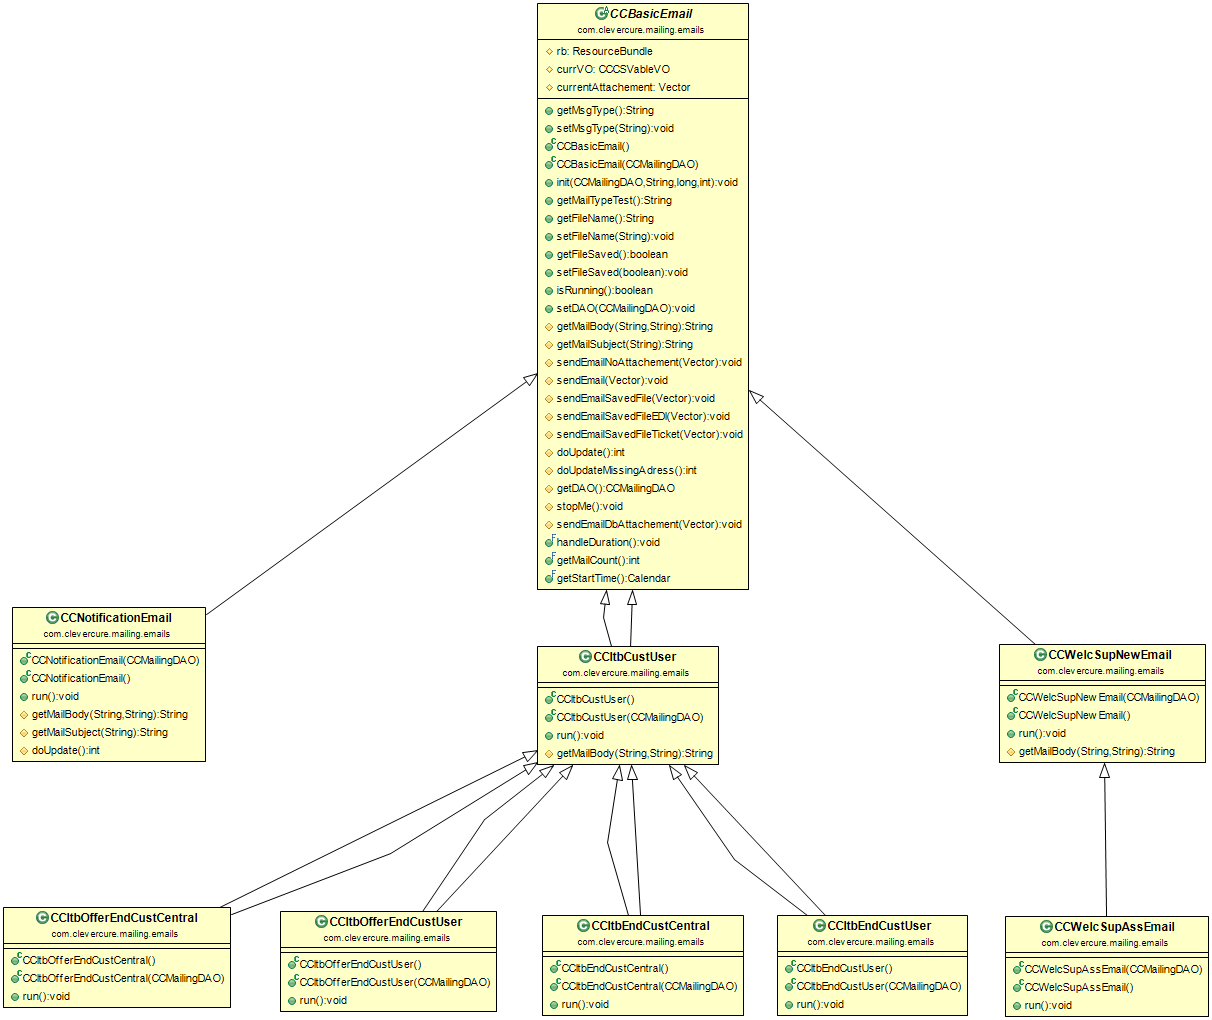
\includegraphics[scale=0.55]{class_diagram_basic_email.png} 
\caption{Auszug aus der Klassenhierarchie von \emph{CCBasicEmail}}
\label{fig:klassen-hierarchie-ccbasicemail}
\end{figure}
\ \newline
Aus diesem Klassendiagramm lässt sich ableiten dass man sich dazu entschieden hat die einzelnen E-Mail-Typen als eigene Klassen abzubilden. Somit ist jeder E-Mail-Typ auch als eigener Java-Typ abgebildet. Am Beispiel der Klasse \emph{CCItbCustUser} ist ebenso ersichtlich dass neben dem Abbilden eines E-Mail-Typs als eigene Java Klasse man ebenfalls eine eigene Subklassenhierarchie eingeführt hat, um E-Mail-Typen, die sich in einem gemeinsamen Kontext befinden, zu gruppieren. Ob dies ein guter Ansatz ist um kontextabhängige Ressourcen zu gruppieren ist zu hinterfragen. Es gäbe hier andere Ansätze wie man eine solche Gruppierung hätte realisieren können, die flexibler sind als eine Klassenhierarchie. Eine Klassenhierarchie ist an sich starr und nicht flexibel und Änderungen an der Struktur können sich negativ auf die Gesamtstruktur auswirken. Ebenso produziert man so eine Vielzahl von Klassen, die gewartet werden müssen und die Struktur einer Subklassenhierarchie lässt sich nur über ein Klassendiagramm darstellen und ist an sich nicht aus dem Source abzuleiten. Ebenso wird man bei den Klassenhierarchien schnell an Grenzen stoßen, da hier nur ein gerichteter Graph abgebildet werden kann und Mehrfachvererbung von Java nicht unterstützt wird. Mehrfachvererbung, auch wenn unterstützt, ist zu vermeiden, da hier Kollisionen bei den Klassenvariablen und Methoden auftreten können. Außerdem wird durch den Einsatz von Mehrfachvererbung die Komplexität der Klassenhierarchie nur unnötig erhöht und bringt daher keinerlei Erleichterungen mit sich.

\subsection{CCItbCustUser}
Nachdem die Klassenhierarchien von \emph{CCBasicEmail} diskutiert wurden wird im folgenden als Beispiel die Implementierung der Klasse \emph{CCItbCustUser} angeführt. Diese Implementierung dient als Beispiel für die restlichen E-Mail-Typ Implementierungen, die nach dem selben Prinzip mit ähnlichen Umfang implementiert wurden. Im Punkt~\ref{sec:implementierung-ccbasic-mail} wurde behauptet dass diese Ableitungen eingeführt wurden um E-Mail-Typen zu gruppieren. Man könnte aber auch davon ausgehen, dass diese eigene Subklassenhierarchie eingeführt wurde, um gemeinsame Funktionalitäten für die abgeleiteten E-Mail-Typen zu kapseln. 
\newline
\newline
Folgender Source-Code illustriert dass die Implementierungen der einzelnen E-Mail-Typen hauptsächlich nur aus dem Aufbau der eigentlichen Nachricht besteht. Die Parameter für die Vorlage werden aus dem Resultat der spezifischen SQL-Abfrage extrahiert und in der Nachricht bzw. der verwendeten Vorlage verwendet. Die erstellte Nachricht wird dann als Resultat zurückgeliefert. Dies ist also der Grund für das Abbilden der einzelnen E-Mail-Typen als eigene Java Klassen. Dieser Ansatz produziert eine Unzahl an Klassen, die in einer starren Hierarchie gebunden sind. Und dies nur um das Erstellen der eigentlichen E-Mail-Nachricht in einer eigenen Klasse bzw. einem eigenen Java-Typ zu kapseln. Es sei angemerkt das diese Klassen auch dazu verwendet um die E-Mail-Typen zu steuern. Die Steuerung beschränkt sich hier aber lediglich auf das Aktivieren und Deaktivieren der E-Mail-Typen. Zu kritisieren ist hierbei dass das Erstellen einer E-Mail-Nachricht zu stark an einen E-Mail-Typ gekoppelt ist und es hier an Abstraktion fehlt. Die E-Mail-Nachrichten werden immer nach dem selben Schema erstellt. Es gibt lediglich nur folgende Unterschiede:
\begin{itemize}
	\item SQL-Abfrage, die die Daten aus der Datenbank bezieht
	\item Die zugrunde liegende E-Mail-Vorlage
	\item Die Paramter für die zugrunde liegende E-Mail-Vorlage
	\item Der eindeutige Schlüssel, der den E-Mail-Typ identifiziert
\end{itemize}
\begin{program}
\caption{Implementierung \emph{CCItbCustUser}}
\label{CCItbCustUser.java}
\begin{JavaCode}
public class CCItbCustUser extends CCBasicEmail {
	
	private Map cache = new HashMap();

	public CCItbCustUser() {
		super();
	}
	
	// sets the used dao implementation
	public CCItbCustUser(CCMailingDAO dao) {
		super(dao);
	}

	// The unique key for this email type
	@Override
	String getMailType() {
		return "ISCU";
	}	
	
	// Thread\#run method which creates and sends the email
	@Override
	public void run() {
		try {
			sendEmailNoAttachement(getDAO().getItbStartCustUserMailText());
		} catch (DAOSysException ex) {
			LOG.error("DAOSysException in CCItbCustUser.run: ",
					   ex);
		} finally {
			stopMe();
		}
	}	
	
	// Method which creates the email body
	@Override
	protected String getMailBody(String bodyKey, String bodySQLKey)
		throws DAOSysException {
		int lanId = ((CCItbVO)currVO).getLanguageId();
		int itbhId = ((CCItbVO)currVO).getItbhID();
		String body = "";
		String key = itbhId	+ "_" + lanId;
		if (cache.containsKey(key)) {
			body = (String) cache.get(key);
			LOG.debug("48: Got from cache key: " + key 
					  + " body: " + body);
		} else {
			Object [] allParams = getDAO().getItbCustData((CCItbVO)currVO, 19);
			MessageFormat form = new MessageFormat(rb.getString(bodyKey)
			                                         .trim());
	 		body = form.format(params);
	 		cache.put(key, body);
	 		LOG.debug("48: DB access for the key: " + key
	 				+ " got body: " + body);
		}
		return body;
	}
}
\end{JavaCode}
\end{program}
\newpage
Die einzelnen E-Mail-Typ Implementierungen implementieren lediglich die folgenden drei Methoden:
\begin{enumerate}
	\item\emph{getMailType}
	\newline
	Bereitstellen eines eindeutigen Schlüssels, der diesen E-Mail Typ identifiziert
	\item\emph{getMailBody}
	\newline
	Erstellen der E-Mail Nachricht aus einer Vorlage, welche mit Parametern befüllt wird
	\item\emph{run}
	\newline
	Jeder E-Mail-Typ wird in einem eigenen Thread abgearbeitet. Hier wird entschiedenen welche Art von E-Mail Versand genutzt wird. \emph{CCBasiEmail} stellt mehrere Implementierungen zur Verfügung wie z.B.:
	\begin{itemize}
		\item Ohne Anhänge
		\item Mit Anhängen, welche über das lokale Filesystem zur Verfügung gestellt werden
		\item Mit Anhängen, welche über externe Systeme zur Verfügung gestellt werden
	\end{itemize}
\end{enumerate}
\ \newline
Dieses Code-Beispiel illustriert das die E-Mail-Typen keine nennenswerte implementierte Logik beinhalten, sondern lediglich für das Erstellen der E-Mail-Nachricht verantwortlich sind. 

\subsection{CCMailingDao}
Im Gegensatz zur Strukturierung der E-Mail-Typen hat man sich bei der Datenzugriffsschicht nicht dazu entschieden diese kontextabhängig zu gruppieren bzw. aufzutrennen. Hier wurden alle Datenbankabfragen in einer einzigen Schnittstelle spezifiziert ohne Rücksichtnahme auf deren Kontext.
\newline
\begin{figure}[h]
\centering
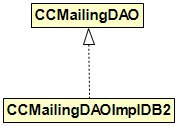
\includegraphics[scale=0.55]{class_diagram_mailing_ao.png} 
\caption{Klassenhierarchie von \emph{CCMailingDao}}
\label{fig:klassen-hierarchie-ccmailingdao}
\end{figure}
\ \newline
Diese Klassenhierarchie ist sehr einfach, da man sich hier nicht für eine Aufteilung der Datenbankzugriffsschicht für die einzelnen E-Mail-Typen entschieden hat. Hier ist zu bemängeln dass sich hier alle Datenbankabfragen über alle E-Mail-Typen hinweg befinden und man es versäumt hat hier Schnittstellen einzuführen, die die kontextabhängigen Datenbankabfragen spezifizieren. Also eine Schnittstelle für jeden E-Mail-Typ. Mit einer Aufteilung auf mehrere Schnittstellen hätte man es sich vereinfacht die Datenbankabfragen zu warten. Mit diesem Ansatz ist man erstens gezwungen Präfixe für die Methodennamen einzuführen, da Namenskollisionen sehr wahrscheinlich sind und zweitens muss man darauf Acht geben bestehende Implementierungen bei einem Refaktorisieren einer oder mehrerer kontextabhängigen Implementierungen nicht zu verändern. Alle Implementierungen nutzen dieselben Ressourcen und müssen daher auf den kleinsten gemeinsamen Nenner zusammengeführt werden, oder man führt hier wiederum eigene Ressourcen ein, die sich durch ihren Namen unterscheiden. Eigene Schnittstellen und Implementierungen je E-Mail-Typ hätten es ermöglicht für diesen E-Mail-Typ Ressourcen zur Verfügung zu stellen, die nur dieser E-Mail-Typ verwendet. Mann hätte Flexibilität erhalten und hätte sich trotzdem auf eine gemeinsame Basis einigen können. Der Ansatz die Implementierungen von \emph{CCMailingDAO} für verschiedene Datenbanken zu zur Verfügung zu stellen ist an sich gut, jedoch hätte man sich mit der Nutzung eines ORM-Mappers (Object-Relational-Mapping) das Leben erleichtern können, da diese ORM-Mapper bereits die zugrunde liegende Datenbank abstrahieren. Datenbank spezifische SQL-Anweisungen und Funktionalitäten werden zwar von den ORM-Mappern nicht zur Verfügung gestellt, jedoch sind solche spezifischen Teile in \emph{CCMail} nicht zu finden. Dieses Feature hätte man schon vor langer Zeit implementieren können, jedoch hat man dies nicht getan. Die Entscheidung sich hier auf native SQL-Abfragen zu stützen bring das Problem mit sich, dass die zugrunde liegende Datenbank nicht von der Anwendung abstrahiert ist und man sich so an eine spezielle Datenbankimplementierung bindet.

\subsection{CCMailingDaoFactory}
Zu kritisieren ist hier auch die Art und Weise wie eine Instanz von \emph{CCMailingDao} erzeugt wird. Man nutzt hier den Factory-Pattern, jedoch wird hier statisch die zu verwendende Implementierung in \emph{CCMailingDaoFactory} definiert, was das Austauschen der Implementierung unmöglich macht. Man hätte dies Konfigurierbar machen sollen z.B.: über eine Konfigurationsdatei, die den zu verwendenden Implementierungsnamen zur Verfügung stellt.
\begin{figure}[h]
\centering
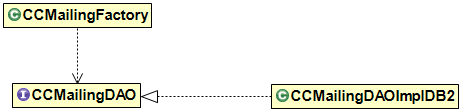
\includegraphics[scale=0.55]{class_diagram_mailing_dao_factory.png} 
\caption{\emph{CCMailingDaoFactory} für \emph{CCMailingDao}}
\label{fig:klassen-hierarchie-ccmailingfactory}
\end{figure}
\ \newline 
In dem Buch \emph{Refactoring to patterns} \cite[72]{refactoreToPatterns} wird als Nachteil einer Factory die erhöhte Komplexität des Designs genannt, wenn eine direkte Instanziierung auch genügen würde. Nachdem die Instanziierung in der Basisklasse \emph{CCBasicEmail} erfolgt und die Ableitungen die Instanz über eine Getter-Methode oder die geschützte Member-Variable erreichen können, hätte man auf diese Factory verzichten können, da die Abstraktion bereits über die Basisklasse \emph{CCBasiEmail} erreicht wurde. Somit ist der Formalparameter der Constructoren vom Typ \emph{CCMailingDAO} sinnlos und der Grund warum man dies eingeführt hat ist nicht ersichtlich. Man hätte die Verwaltung der \emph{CCMailingDAO} Instanz in der abstrakten Basisklasse \emph{CCBaisEmail} halten sollen ohne die abgeleiteten Klassen damit zu verschmutzen. 
\newline 
\newline
Zusätzlich befindet sich die Schnittstelle zusammen mit ihrer Implementierung in ein und demselben Artefakt. Dies ist auch als ein halbherziger Versuch zu werten die Implementierung von \emph{CCMailingDao} austauschbar zu machen. Man hätte hier die Schnittstellen und Implementierungen auf eigene Artefakte aufteilen sollen. Somit hätte man die Abhängigkeit zu der konkreten Implementierung vermieden und hätte sich nicht der Gefahr ausgesetzt, dass ein Entwickler sich direkt auf die Implementierung beziehen könnte und daher immer gezwungen wäre mit den Schnittstellen zu arbeiten.
\newpage
\section{Datenbank}
\label{sec:ccmail-datanbank}
Abschließend wird hier der Aufbau des Datenbankschemata betrachtet, welches die Kernkomponente des Systems aus der Sicht von \emph{CCMail} darstellt. Es wurde bei diesem Schemata offensichtlich auf Fremdschlüssel verzichtet, was grundsätzlich nur in Spezialfällen anzuraten ist. In dem Buch \emph{Refactoring Database} \cite[213]{refactoreDatabase} wird als Argument für nicht verwendete Fremdschlüssel die Performance genannt, wobei in diesem Fall diese Begründung nicht standhält. Die beiden Anwendungen \emph{CleverWeb} und \emph{CleverInterface} erstellen lediglich einzelne oder wenige \emph{MailJob} Einträge auf einmal und \emph{CCMail} ist die einzige Anwendung, die diese \emph{MailJob} Einträge einmalig ausliest und verarbeitet. Also sollte in diesem Fall die Performance ohnehin kein Problem darstellen, da hier eine Vielzahl von Teilnehmer und die dadurch resultierende Konkurrenz nicht geben ist. Das Problem von nicht verwendeten Fremdschlüsseln wird in \emph{Refactoring Databases} \cite[213]{refactoreDatabase} wie folgt beschrieben.
\begin{quote}
\emph{The fundemental tradeoff is performance versus quality: Foreign key constraints ensure the validity of the data at the database level at the cost of the constraint being enforced each time the source data is updated. When you apply Drop Foreign Key, your applications will be at risk of introducing invalid data if they do not validate the data before writing to the database.}
\end{quote}
Hier müssen also die Anwendungen selbst die Konsistenz der Daten gewährleisten ansonsten könnten inkonsistente Datenbestände in der Datenbank entstehen, die nachträglich schwer zu identifizieren und zu bereinigen sind. Die Frage ist hierbei ob dieser Ansatz ein guter Ansatz ist?
\newline
\newline
Wie auch ersichtlich ist wurden die Spalten einer Tabelle mit einem Präfix versehen, der eindeutig über das gesamte Datenbankschema ist. Mann sollte annehmen dass es ausreicht dass die Spaltennamen eindeutig innerhalb des Kontextes einer Tabelle sind und nicht global über das gesamte Datenbankschema. Die Tabellen die neu eingeführt wurden und mit Fremdschlüsseln miteinander verknüpft sind werden dazu verwendet um Datei Anhänge von E-Mail-Nachrichten zu verwalten, die bereits bei der Erstellung des \emph{MailJob} erstellt wurden. Dies war ein Workaround und sollte so auch nicht mehr angewandt werden, da hier die Dateien in Base64 Kodierung verwaltet werden und die Datenbank unnötig mit Daten belasten. Sie sollten in einem File-Storage verwaltet und lediglich referenziert werden, was aber zum Zeitpunkt der Implementierung noch nicht zur Verfügung stand. 
\begin{figure}[h]
\centering
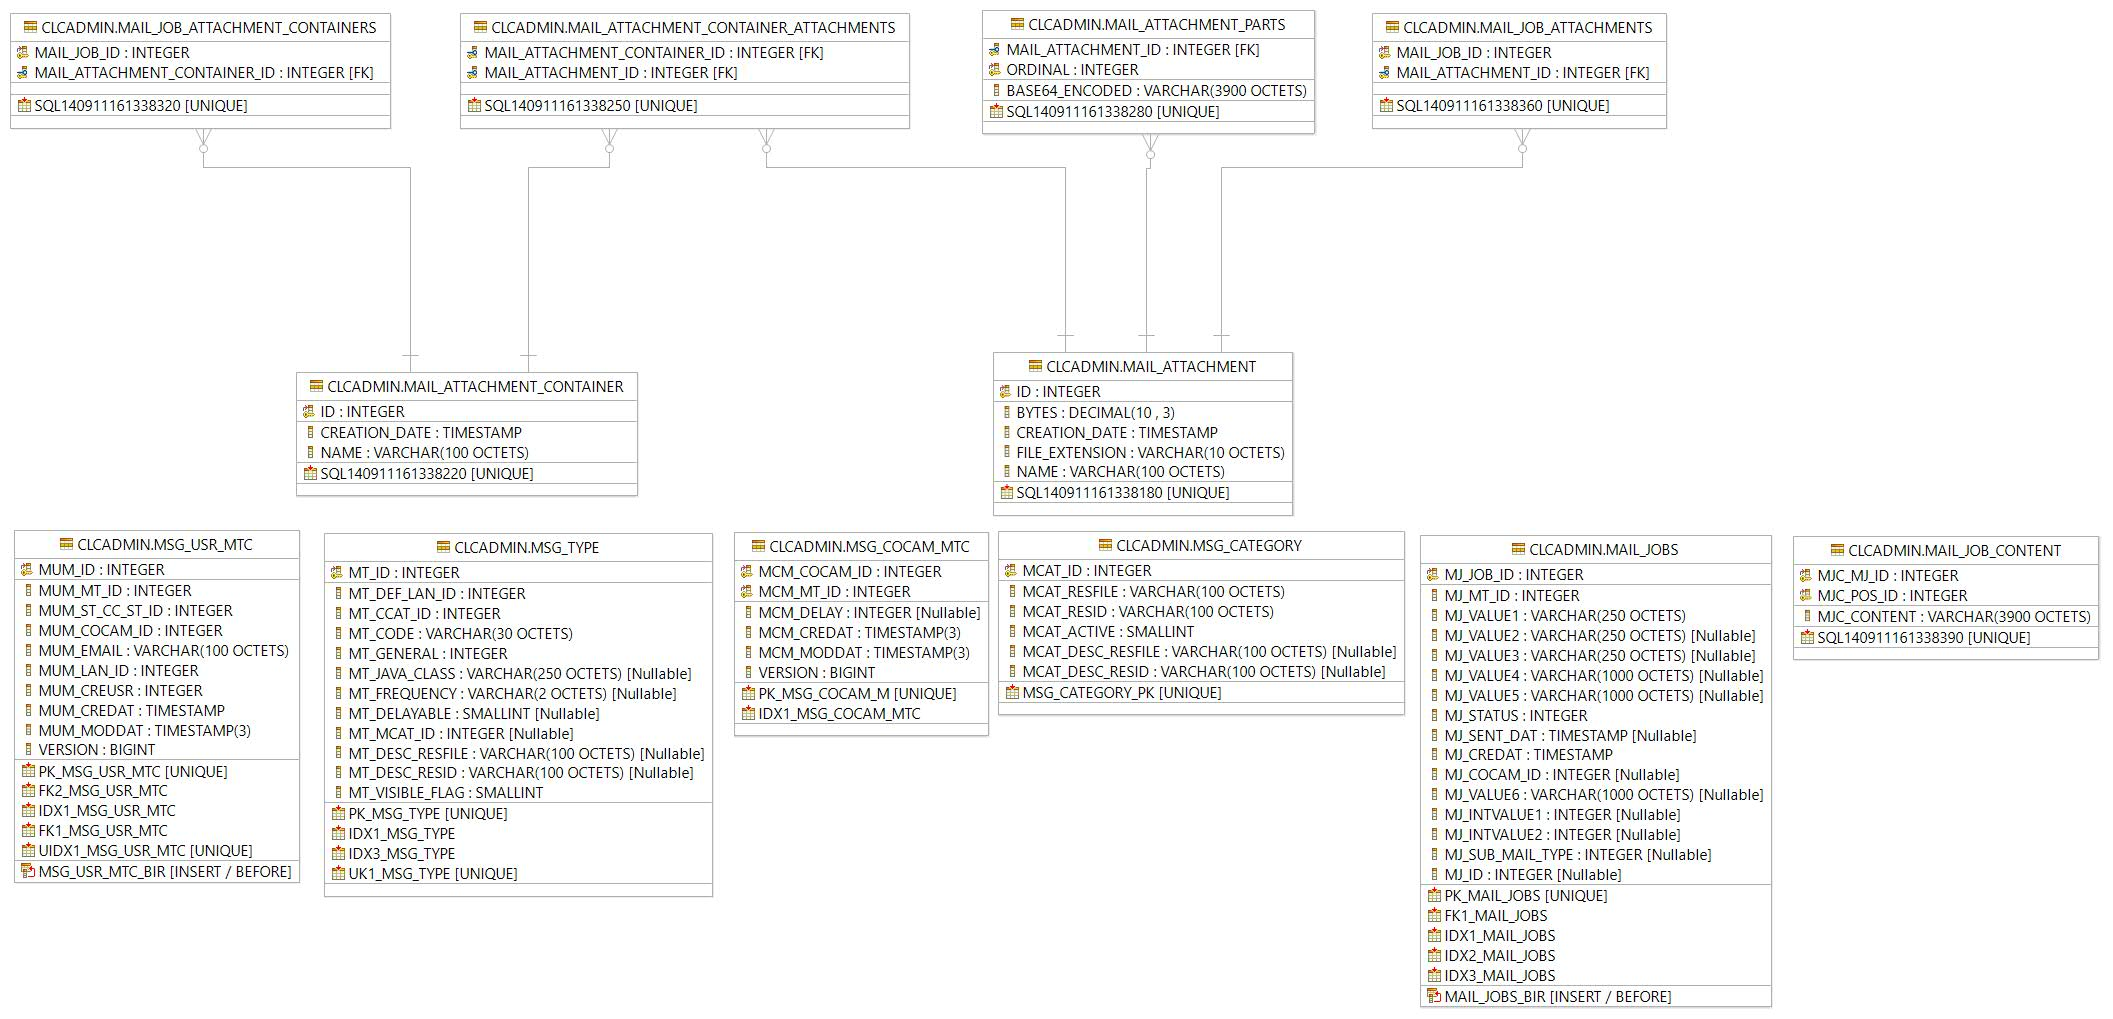
\includegraphics[angle=90,scale=0.3]{ccmail_db_schema.jpg} 
\caption{Datenbankschemata \emph{CCMail}}
\label{fig:ccmail-db-schema}
\end{figure}
